\chapter{Extra-Credit Question-5}
\label{intro}

\textbf{ Re-run question 2, but this time with proper TFIDF calculations instead of the hack discussed on slide 7 (p. 32).  Use the same 500 words, but this time replace their frequency count with TFIDF scores as computed in assignment 3.  Document the code, techniques, methods, etc. used to generate these TFIDF values.  Upload the new data file to github.\\\\
Compare and contrast the resulting dendrogram with the dendrogram from question 2.\\\\
Note: ideally you would not reuse the same 500 terms and instead come up with TFIDF scores for all the terms and then choose the top 500 from that list, but I'm trying to limit the amount of work necessary.}\\


Following are the steps I have taken to solve the problem:

\begin{itemize}
\item I calculated the TFIDF values similar to assignment 3.
\item I got the JPEG dendogram using the same python code as question 2 \ref{lst:q5code1} 
\newpage
\item The output JPEG that clusters the most similar blogs based on TFIDF values is illustrated in the Figure \ref{fig:q5fig1}
\begin{figure}[h!]
\begin{center}
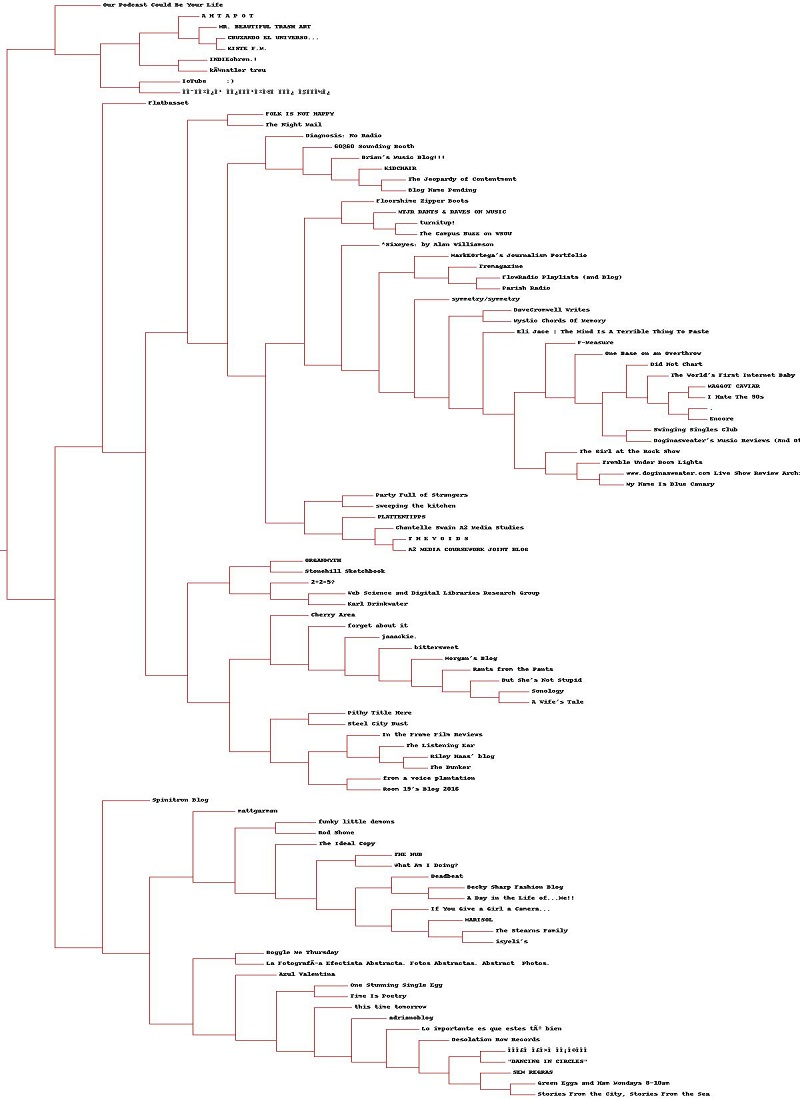
\includegraphics[scale=0.55, keepaspectratio=true]{figures/blogclust1.jpg}
\caption{JPEG dendogram}
\label{fig:q5fig1}
\end{center}
\end{figure}
\item Therefore I generated the output file `blogdataWithTFIDF.txt' which has a blog matrix with blog title as identifier for each blog. This text file is uploaded to github at \url{https://github.com/majetisiri/cs532-s16/blob/master/a8/q5-blogdataWithTFIDF.txt}
\item By comparing and contrasting we can say that the blog dendogram based on TFIDF has more clusters than the blog dendogram with frequency count in question 1. By looking at the dendograms it seems there is a much difference, only the hierarchy of clusters are changing but the clusters are around the same blog with different hierarchy. This is illustrated in Figure \ref{fig:q5fig2}.
\begin{figure}[h!]
\begin{center}
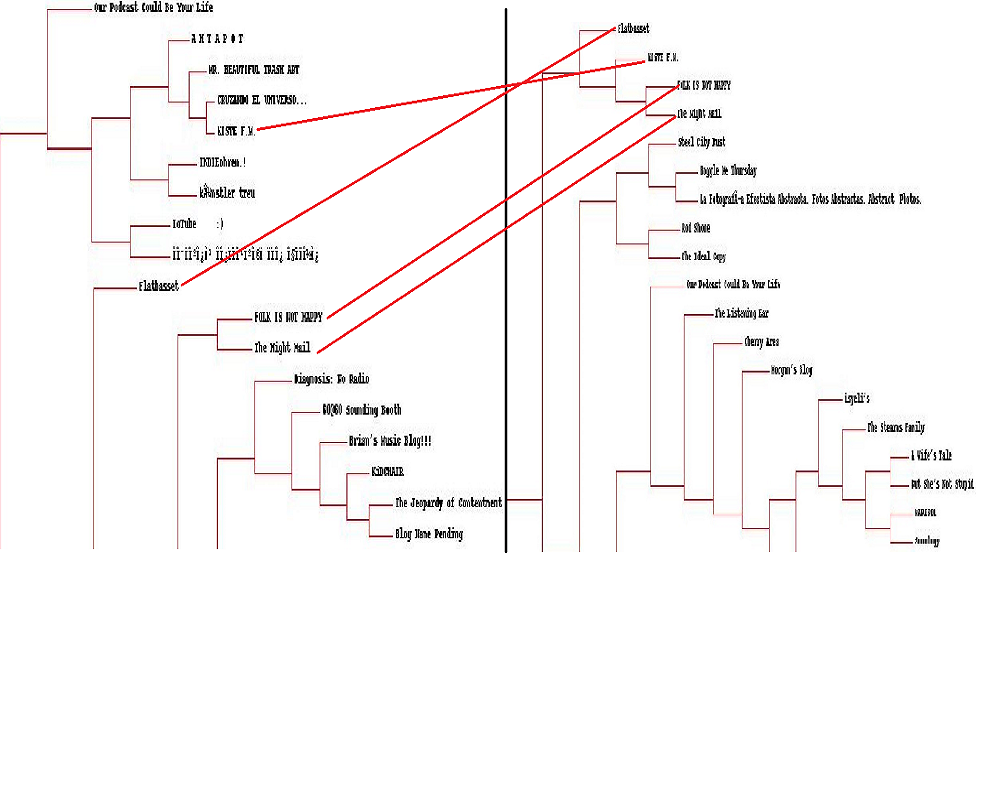
\includegraphics[scale=0.55, keepaspectratio=true]{figures/combined.png}
\caption{comparing and contrasting dendograms from question 1 and question 5}
\label{fig:q5fig2}
\end{center}
\end{figure}
\end{itemize}


\newpage
\textbf{Code Listing}
\sloppy
\lstinputlisting[language=Python,caption=Python code for calculating TFIDF,frame=single,breaklines=true,label=lst:q5code1, tabsize=2, captionpos=b,numbers=left,showspaces=false,showstringspaces=false,basicstyle=\footnotesize]{src/getTFIDF.py}

